\clearpage

\hypersetup{linkcolor=black}
\tableofcontents % Prints the main table of contents
\hypersetup{linkcolor=blue}
\renewcommand\arraystretch{1}

\listoffigures
\listoftables

\begin{abbreviations}{ll}

\textbf{APT} & Advanced Persistent Threat\\
\textbf{AST} & Abstract Syntax Tree\\
\textbf{CI/CD} & Continuous Integration / Continuous Deployment\\
\textbf{CISA} & Cybersecurity and Infrastructure Security Agency\\
\textbf{CPE} & Common Platform Enumeration\\
\textbf{CVE} & Common Vulnerabilities and Exposures\\
\textbf{DDoS} & Distributed Denial of Service\\
\textbf{eBPF} & Extended Berkeley Packet Filter\\
\textbf{MFA} & Multi-Factor Authentication\\
\textbf{MALOSS} & Malware detection for Open Source Software\\
\textbf{NVD} & National Vulnerability Database\\
\textbf{SBOM} & Software Bill of Materials\\
\textbf{SMT} & Satisfiability Modulo Theories\\

\end{abbreviations}

\begin{symbols}{lll}

$G=(V,E)$ & Dependency graph of package ecosystem & -- \\
$V$ & Set of package nodes & -- \\
$E$ & Set of dependency edges & -- \\
$d$ & A dependency in the project dependency set & -- \\
$P$ & Security policy rule set & -- \\
$T$ & Trusted source and provenance map & -- \\

\addlinespace 

$\rho(d)$ & Risk score assigned to dependency $d$ & -- \\

\end{symbols}

\mainmatter % Begin numeric (1,2,3...) page numbering
\pagestyle{thesis} % Return the page headers back to the "thesis" style

\chapter{Introduction}
\label{ch:introduction}

Modern systems rely heavily on secure digital infrastructure globally. Organisations have started using cloud services and automated systems. This amplifies the frequency and complexity of cyber threats. Today, attack vectors are not just independent hackers, doing things for fun; rather they range from well formed criminal syndicated to state sponsored groups. With increasing financial impact of cyberattacks, organisations have to completely rethink the way they approach cybersecurity.

Earlier, systems were limited to individual organisations and hence threats could be mitigated by just a single firewall. Over time, networks began to span all over the world and these defence systems have improved significantly. Attackers have also shifted their tactics. Instead of direct attacks, they now focus on the gaps between the implementation and the foundations of the software itself.

This shift in tactics has exposed a major weakness in modern technology - the software supply chains. Developers no longer write entire programs from scratch, rather they rely on a huge network of third party, open-source code libraries and public package managers. These systems are highly interconnected and relies mostly on ‘trust’. By compromising just one trusted component, attackers can insert harmful code in the source packages. These altered softwares are distributed and the hidden malware spreads silently over the whole interconnected network. Traditional security measures fall inadequate in these situations.

To explore this growing challenge in more detail, we first give a broad view of cybersecurity threats and gradually shift our focus to the supply chain vulnerabilities. We begin by outlining the major types of cyber threats seen today. The discussion then narrows to examine the specific methods attackers use to compromise software supply chains. To get familiar with the situation, we present a recent case study involving this attack. Finally, the report details practical defence strategies. By exploring concepts like Zero-Trust models, pipeline security, and code verification, the report outlines how organisations can protect their software development lifecycles against these widespread, modern threats.

\chapter{Background: Overview of the Modern Cyber Threat Landscape}
\label{ch:threat-overview}

\section*{Declaration of Contributions}
This chapter was prepared primarily by Adesh Palkar, with technical inputs from all Group 4 members.
The threat taxonomy and mitigation mapping were consolidated jointly during group reviews.

\section{Background}
The digital security landscape has become an organised and highly profitable criminal system. According to the Microsoft Digital Defense Report, malicious activity has reached record levels. Password attacks happen at a rate of over 4,000 per second, and over 65 trillion threat signals are analysed daily \cite{mddr_2023}. Today's attackers are not just random hackers. They include well funded government teams known as Advanced Persistent Threats (APTs) and organised crime groups.

As companies rely more on digital tools, the attack surface has grown rapidly. Vulnerabilities now exist across cloud systems, CI/CD pipelines, open source code networks, and smart devices (IoT). Because of this, modern attacks are highly targeted and difficult to remove. Attackers link multiple techniques along the cyber kill chain to reach their goals.

\section{Major Cyber Threat Categories}
Although there are many types of threats, adversarial actions typically fall into a few main groups. We survey six primary threat vectors before detailing our focal concern: software supply chain attacks  \cite{enisa_etl_2023}.

\begin{description}
    \item[1. Malware and Ransomware] \hfill \\
    Malware includes executables, macros, and downloads designed to encrypt, exfiltrate, or destroy data. Ransomware as a Service (RaaS) makes it easy for even low skill actors to launch ransom attacks.
    
    \textit{Mitigation:} Deployment of Endpoint Detection \& Response (EDR) solutions alongside offline, locked data backups. Regularly testing the restoration process from these backups is key to quick recovery during an incident.

    \item[2. Phishing and Social Engineering] \hfill \\
    Social engineering initiates most successful data breaches \cite{verizon_dbir_2023}. It tricks human psychology using emails, SMS, or voice calls to steal credentials or install malware. Spear phishing uses background research to make emails look real.
    
    \textit{Mitigation:} FIDO2 hardware tokens for MFA and strong email rules (DMARC, DKIM, SPF). Simulating fake phishing exercises continuously helps to measure and reinforce employee vigilance against evolving deceptive tactics.

    \item[3. Zero Day Exploits] \hfill \\
    This attacks involves exploiting unknown or unpatched software vulnerabilities before the vendor has issued a fix. Hackers buy and sell these zero days to break into systems quietly or gain higher access levels.
    
    \textit{Mitigation:} Use Web Application Firewalls (WAF/IPS) for virtual patching, run bug bounty programs, and continuously test code. Isolating legacy or critical systems through strict network micro segmentation significantly limits the lateral movement of an attacker who successfully breaches the perimeter.

    \item[4. Man in the Middle Attacks] \hfill \\
    Attackers intercept or change data as it travels using methods such as ARP spoofing and DNS cache poisoning. These are major risks in modern cloud services.
    
    \textit{Mitigation:} Enforce TLS 1.3 encryption and adopt a Zero Trust Network Architecture (ZTNA). Pinning digital certificates inside corporate apps helps block rogue access points or compromised routers from reading the traffic.

    \item[5. DDoS Attacks] \hfill \\
    Distributed Denial of Service blocks real users by flooding systems with junk internet traffic. Attackers leverage open internet resolvers (such ad DNS, NTP) to multiply the attack size.
    
    \textit{Mitigation:} Distribute traffic using Anycast, use robust CDN scrubbing, and set up BGP blackholing. failover mechanisms to geographically distributed data centres ensures keep services online during long attacks.

    \item[6. Insider Threats and Credential Abuse] \hfill \\
    These threats originate from malicious or negligent actors who possess legitimate access to systems. The risk is high in DevOps environments where many users have high level rights.
    
    \textit{Mitigation:} Follow the Principle of Least Privilege (PoLP) and use Privileged Access Management (PAM) frameworks. Checking user activity logs regularly helps spot odd internal actions early before data is lost.
\end{description}

\section{The Focal Threat: Software Supply Chain Attacks}

        \vspace{0pt}
        Unlike the previous attacks that target an organisation's perimeter directly, software supply chain attacks compromise a trusted third party. This could be an open source library, a build tool, or a package registry (like npm or PyPI). Once a malicious payload is successfully injected, it propagates silently and automatically to all downstream consumers at scale.

        \vspace{1em}
        \textbf{The core attack vector is trust itself.} Attackers exploit this trust through a variety of injection methods:
        \begin{itemize}
            \item \textbf{Typosquatting:} Uploading packages with names very similar to popular libraries (e.g., \texttt{reqeusts} instead of \texttt{requests}).
            \item \textbf{Dependency Confusion:} Tricking build systems into downloading malicious public packages instead of safe internal ones.
            \item \textbf{Maintainer Takeover:} Gaining unauthorised access to a legitimate package by phishing or compromising the original author's credentials.
            \item \textbf{Malicious Updates:} Introducing poisoned patches to an otherwise historically trusted and legitimate package.
        \end{itemize}
        
\begin{figure}[htbp]
    \centering
    \begin{minipage}[t]{0.45\textwidth}

        \vspace{1em}
        As shown in Figure \ref{fig:supply_chain_flow}, an attacker does not need to target a specific organisation directly. By poisoning the upstream package repository, the automated CI/CD tools and package managers of all the downstream consumers will unknowingly download and exexute the compromised code during routine processes.
    \end{minipage}\hfill
    \begin{minipage}[t]{0.55\textwidth}
        \vspace{0pt}
        \centering
        \begin{tikzpicture}[
            every node/.style={font=\scriptsize},
            box/.style={
              draw, rounded corners=3pt,
              minimum width=2.0cm, minimum height=0.55cm,
              align=center, fill=blue!10, text=black
            },
            attacker/.style={
              draw, rounded corners=3pt,
              minimum width=1.8cm, minimum height=0.55cm,
              align=center, fill=red!15, text=black
            },
            registry/.style={
              draw, rounded corners=3pt,
              minimum width=2.0cm, minimum height=0.55cm,
              align=center, fill=orange!20, text=black
            },
            consumer/.style={
              draw, rounded corners=3pt,
              minimum width=1.3cm, minimum height=0.5cm,
              align=center, fill=blue!10, text=black
            },
            arr/.style={-{Stealth[length=4pt]}, thick},
            redarr/.style={-{Stealth[length=4pt]}, thick, red!70!black},
            scale=0.75, transform shape
          ]

          % Developer (legitimate)
          \node[box] (dev) at (0, 3.2) {Developer\\(legitimate)};

          % Registry
          \node[registry] (reg) at (0, 1.8) {Package Registry\\(npm / PyPI)};

          % Attacker
          \node[attacker] (atk) at (3.5, 1.8) {Attacker};

          % Package manager
          \node[box] (pm) at (0, 0.4) {\texttt{pip install} /\\\texttt{npm install}};

          % Consumers
          \node[consumer] (c1) at (-2.0, -1.0) {Org A};
          \node[consumer] (c2) at (0,   -1.0) {Org B};
          \node[consumer] (c3) at (2.0, -1.0) {Org C};

          % Arrows
          \draw[arr] (dev) -- node[right, xshift=2pt]{publishes} (reg);
          \draw[redarr] (atk) -- node[above, yshift=2pt]{\textcolor{red!80!black}{injects}} (reg);
          \draw[arr] (reg) -- node[right, xshift=2pt]{trusted pull} (pm);
          \draw[arr] (pm) -- (c1);
          \draw[arr] (pm) -- (c2);
          \draw[arr] (pm) -- (c3);

          % Poison label on registry
          \node[font=\tiny, red!70!black, align=right] at (-1.3, 1.1)
            {poisoned package \Large $\searrow$};

        \end{tikzpicture}
        \caption{Software Supply Chain Attack Flow}
        \label{fig:supply_chain_flow}
    \end{minipage}
\end{figure}

\chapter{XZ Utils Backdoor (2024): A Software Supply Chain Case Study}
\label{ch:casestudy}

\section*{Declaration of Contributions}
This chapter was prepared by Nisarg Prajapati, with final review by the group.

\section{Introduction to the Incident}

The XZ Utils backdoor stands as one of the most obvious contemporary instances of a software supply chain security breach. It functions as a popular compression tool for Linux systems which many software environments use through its \texttt{liblzma} library. The incident reached its most critical point because of two factors, which included the introduction point of malicious code and its development origin. The upstream release process for version 5.6.0 and version 5.6.1 included the compromise, which appeared at a location that downstream users regarded as secure and reliable. 

The XZ incident demonstrated how software supply chains can be targeted through intentional design, which creates security vulnerabilities that differ from typical programming mistakes. Public analysis showed that the malicious release artifacts triggered build time behavior that differed from what many reviewers would expect by looking only at the visible source tree. Security review requires both release artifacts and build behavior to undergo verification \citep{nvd2024cve3094,redhat2024xz}.

\section{Discovery and Why It Was a Near Miss}

The incident came to light only after unusual system behavior was noticed. Andres Freund reported abnormal symptoms on Debian sid systems, including unexpectedly high CPU usage during SSH logins and unusual Valgrind output. Those anomalies led to deeper investigation, which ultimately exposed the upstream compromise and triggered public disclosure on 29 March 2024 \citep{freund2024xz}.

This event is often described as a near miss because the most dangerous forms of the compromise had not yet spread deeply across stable enterprise environments at the time of disclosure. In other words, the wider ecosystem was not protected by strong default trust controls alone. It was protected largely because suspicious operational symptoms were identified early enough to interrupt further downstream propagation. That makes the XZ incident not only a case of malicious code insertion, but also a warning about how close ordinary software distribution channels came to carrying a dangerous backdoor.

\section{Technical Nature of the Compromise}

Modern software systems demonstrate extended attack surfaces that exceed application source code protection. The compromise did not rely on a conventional exploit such as a direct memory corruption bug in a network facing service. The system used its trust relationship with its release and build pipeline process. The attacker used the upstream packaging process to install backdoor access, which infected systems through their regular installation and update processes.

Supply chain attacks fundamentally differ from direct attacks because their execution requires different methods. The attacker does not need to compromise every target one by one. Instead, one shared dependency becomes the delivery path for many possible victims. It is a strong example of this risk because it is a low level component.

\begin{figure}[htbp]
\centering
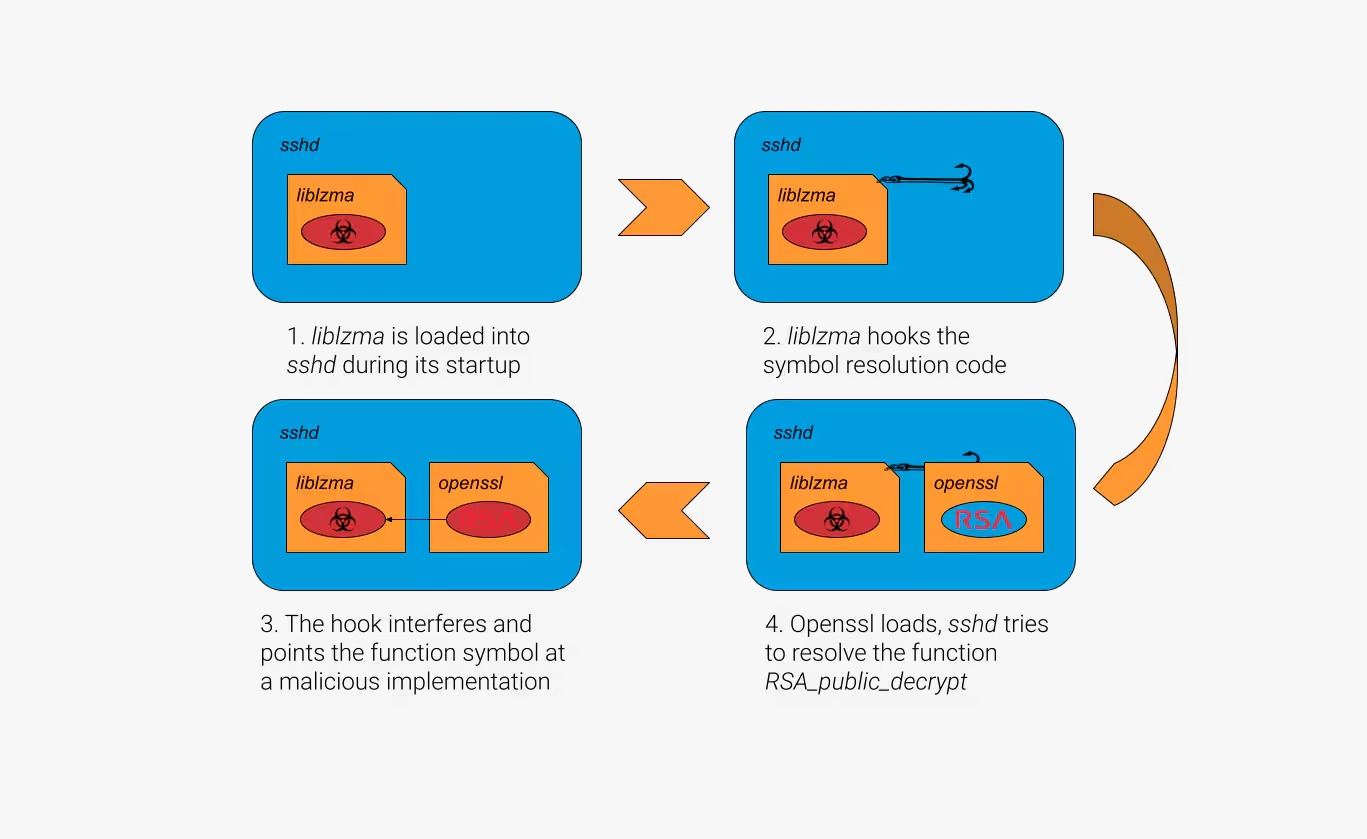
\includegraphics[width=0.82\textwidth]{imgs/image3.jpeg}
\caption{Simplified \texttt{liblzma} hooking process in the XZ Utils backdoor \citep{akamai2024xz}.}
\label{fig:xz-hooking}
\end{figure}

Figure~\ref{fig:xz-hooking} illustrates the technical mechanism in simplified form. The compromised \texttt{liblzma} library interferes with symbol resolution during loading, allowing it to redirect a sensitive OpenSSH related function toward malicious behavior. This figure is useful because it makes clear that the incident was not a normal SSH bug. Instead, it was a dependency level compromise affecting a trusted library path.

\section{Governance and Trust Lessons from the Case}

The XZ incident demonstrated a governing issue which extended beyond its technical difficulties. Software supply chain security requires more than automated code analysis and code scanning. The project needs security through its release governance and its maintainer base and its relationships which exist among its open source members.

The evaluation of dependencies needs to consider more than the two metrics of usage and community recognition. Organizations should also ask whether a project has transparent release practices, active review controls, clear maintainer accountability, and evidence that published
artifacts match reviewed source. The XZ case demonstrates that attackers spend time building their authority and control before they start their technical attacks.

\section{Key Lessons from the XZ Case}

The XZ incident highlights several practical lessons for software supply chain security:

\begin{itemize}
    \item Historical dependency reputation should not establish trust toward dependencies.
    \item Organizations should handle release artifacts as security sensitive elements.
    \item Security assessments need to cover all components of build pipelines since they function as attack surfaces.
    \item Users do not see low level packages yet these packages create security threats which affect the entire system.
    \item Governance weakness can be as dangerous as code weakness.
\end{itemize}

The XZ incident should not be considered an independent security breach because these details demonstrate. The evidence shows that software ecosystems today need better methods to establish and maintain trust between systems.

\chapter{Problem Statement and Security Implications}
\label{ch:problem}

\section*{Declaration of Contributions}
This chapter was prepared by Nisarg Prajapati, with wording review and alignment completed by the group.

\section{Problem Statement}

\begin{quote}
\textbf{The widespread blind trust in unverified open source dependencies exposes organizations to devastating software supply chain attacks.}
\end{quote}

The statement reveals a fundamental structural defect that exists within contemporary software engineering. The majority of organizations today construct their software systems by combining existing software components rather than developing complete systems from their foundation. The developers use third party libraries and packages together with build tools and transitive dependencies to create their software. The development model enables faster development processes while decreasing duplicated work however it introduces security risks because organizations must rely on third party components whose security status they cannot completely assess. The XZ case demonstrates the issue because it reveals how a single trusted upstream dependency breach can lead to extensive security risks throughout the system.


\section{Why Blind Trust Persists in Practice}

A lack of diligence is not always what causes blind trust. In most cases, the source of this trust lies in complex situations where there is little time for proper action and the magnitude of dependencies involved. Programmers typically deal with large dependency trees, quickly changing package repositories, and deadlines. Under such circumstances, software packages get used because they are common or convenient.

It can be challenging too. Application code review can be hard enough, but the analysis of release artifacts, build process, modifications made by maintainers, and transitive dependencies in an extensive dependency graph becomes even tougher. Thus, securing dependencies cannot be equated to selecting a popular package only. Other aspects must be considered as well.

\section{Security Implications for Organizations}

Security concerns are significant because the exploitation of a supply chain is efficient. One tainted component can impact several applications simultaneously if that particular software package is used for development, testing, and production. Additionally, upstream contamination can render local controls irrelevant as malicious activity can be propagated as part of an update process.

From a practical point of view, this implies that the compromise of just one dependency can result in the exposure of several internal systems, that trusted upstream dependencies can undermine local defense mechanisms, and that malicious activity might look like standard releases. In addition, detecting such behavior is made more difficult because the dependency continues to look like a legitimate dependency. On the level of governance, if the organization has no explanation for the source of a particular dependency, its maintenance, its release, and its consistency with the reviewed source, it controls nothing at all.

\section{What This Implies for Defensive Strategy}

Addressing the issue demands more layers of controls beyond a one size fits all security approach. The ideal protection against dependencies should integrate both technological checks and governance controls. Dependencies should be validated regarding their source, ownership, and versioning before they can be adopted or deployed.

Monitoring for any unexpected maintainership or ownership shift, inspecting build and installation instructions in critical packages, and keeping track of dependencies constantly are other measures that need to be considered. Dependency update activity should be seen as a security related event rather than a standard maintenance task. More generally, the key point is that trust needs to be based on facts.

\chapter{Related Work - NDSS Research Paper}
\label{ch:related-ndss}

\section*{Declaration of Contributions}
This chapter was prepared by Utkarsh Kumar covering the sections in this chapter namely: Research Context and Motivation, Attack Path, MALOSS Pipeline, Key Findings, Mitigation Strategies and Limitations

\section{Research Context and Motivation}

Duan \textit{et al.} created the ecosystem level research study which examined the security of software package managers \citep{duan2021ndss}. They developed MALOSS (MALware detection for Open Source Software) as a method which enables researchers to discover malware in packages.

\subsection{What Problem Does the Paper Address?}

Modern software applications require third party libraries which developers obtain from various package repositories like PyPI and npm. This dependency model improves development speed but creates an implicit trust requirement because developers and organizations frequently install and update packages without verifying it.

The NDSS paper shows how attackers use trust to execute their attacks. Instead of directly attacking each target organization, attacker can place malicious logic upstream. Where one successful compromise can propagate to many downstream users.

\subsection{What Does the Paper Aim to Do?}

The study has three main goals: Establish a method to examine security flaws throughout various package ecosystems, Investigate common security issues which include trust assumption failures and recurring vulnerabilities that enable cyberattacks and Creating an automated pipeline named MALOSS which identifies harmful software packages throughout entire software ecosystems.

\section{Attack Path}

The NDSS model describes supply chain compromise as a trust propagation path that extends from package maintainers to registries, from registries to application builders, and finally to end users. Security risk increases because attacks typically enter upstream, where packages are first published and where ecosystem participants often assume legitimacy by default. The development and deployment pipelines operate normally until malicious packages are accepted as standard dependencies which leads to downstream impact throughout the system.

\begin{figure}[htbp]
\centering

\includegraphics[width=0.96\textwidth]{imgs/fig_1.png}
\caption{Package manager ecosystem attack path and trust propagation.
Source: Duan \textit{et al.}, NDSS 2021, Fig.~1 \citep{duan2021ndss}.}
\label{fig:ndss-attack-path}
\end{figure}

The figure displays an attack surface which consists of four distinct points of compromise. The most important practical insight is that downstream teams may inherit risk even when their internal controls are mature, because compromise can be introduced before code reaches their environment. Trust in dependency ecosystems should be continuously verified with policy and evidence, not assumed based on package popularity or historical reputation.

\section{MALOSS Pipeline}

MALOSS operates malware detection through its three step process which combines metadata analysis with code analysis and runtime monitoring and human expert validation. The system architecture enables operation across extensive package networks while maintaining full control of high confidence verification processes for analysts.

\subsection{Metadata Analysis}
The process of metadata analysis provides an low cost method to conduct preliminary assessments. The system investigates various signals which include author, release history, dependency relationships, naming similarity and suspicious references. The current stage enables the identification of typosquatting and suspicious maintainer activities and package anomalies which require further investigation.

\subsection{Static Analysis}
Static analysis scans source and package scripts to detect dangerous API usage and unusual patterns of control and data movement like network access and filesystem manipulation. The system effectively detects suspicious sequences which start with accessing sensitive local data and end with sending data through the network. Static checks provide effective and scalable testing solutions.

\subsection{Dynamic Analysis}
The dynamic analysis process tests software packages in specially designed Docker like sandbox environments which track their execution during specific phases: installation, package importation, and function execution. The system records dynamic execution activities which include DNS and IP address operations, file access through reading and writing. The current phase of the process captures operational activities which remain hidden from static analysis methods.

\subsection{Human in the loop Validation}
The process of human in the loop validation demonstrates which cases need further examination while determining which results are accurate and which results are false alarms. The process of manual triage establishes two benefits because it increases accuracy and enables security teams to trust the pipeline as a reliable operational tool.

\begin{figure}[htbp]
\centering

\includegraphics[width=0.96\textwidth]{imgs/fig_2.png}
\caption{MALOSS pipeline stages\\
Source: Duan \textit{et al.}, NDSS 2021, Fig.~4\citep{duan2021ndss}.}
\label{fig:ndss-maloss-pipeline}
\end{figure}

\section{Key Findings}

The study produced evidence that supply chain attack is measurable and  significant\citep{duan2021ndss}. 

\begin{itemize} \setlength\itemsep{0.2em}\setlength\parskip{0pt}
\item MALOSS analyzed over 1 million packages across PyPI, npm, and RubyGems.
\item It identified 339 new malicious packages, and 278 were later confirmed and removed.
\item Three removed packages had more than 100K downloads and were assigned CVEs.
\item About 20\% of observed malware remained online for over 400 days.
\end{itemize}

\section{Mitigation Strategies}

Some mitigation strategies suggested by authors for stakeholders in the package ecosystem.

\begin{itemize} \setlength\itemsep{0.2em}\setlength\parskip{0pt}
\item \textbf{Registry maintainers:} Enforce MFA, deploy automated vetting, improve typo detection and issue rapid advisories to strengthen ecosystem wide security.
\item \textbf{Package maintainers:} Secure infrastructure, restrict privileged access, and follow safer publishing workflows to prevent compromise.
\item \textbf{Developers and teams:} Pin dependencies, review install/build scripts, and treat dependency updates as security critical events.
\item \textbf{Ecosystem response:} Notify dependents quickly, coordinate takedowns, and manage emergency releases for high impact packages.
\end{itemize}

\section{Limitations}

The paper has some of the limitations found by the writer of this section:

\begin{itemize} \setlength\itemsep{0.2em}\setlength\parskip{0pt}
\item Static and dynamic analysis can produce false positives and miss hidden behaviors.
\item Dynamic analysis depends on execution paths, so trigger based malware can evade detection.
\item Large dependency graphs make complete and continuous analysis difficult.
\item Full automation is not happening due to manual verification step.
\end{itemize}

MALOSS should be used as part of a broader security approach, not relied on alone. Its real value is helping teams continuously find risks, prioritize them, and respond quickly across package ecosystems.


\chapter{Related Work - Dependency Confusion}
\label{ch:related-dependency-confusion}

\section*{Declaration of Contributions}
This chapter was prepared primarily by Tanay Kapadia.

\section{Dependency Managers}

Dependency managers, sometimes referred to as package managers, are tools designed to help you organize and maintain the software installed on your computer \cite{matt2017dependencymanagers}. They keep a reliable record of everything that has been installed, making it straightforward to determine what is already available on your system. Through a package manager, you can install new applications, update existing ones, or cleanly remove software you no longer need.

As the name suggests, package managers work with packages, which are self-contained bundles that typically include program binaries, configuration files, and any supporting resources the software requires. By grouping these components together, a package can be installed, updated, or removed as a single cohesive unit. This simplifies software management considerably and helps ensure that each program's requirements are handled in a consistent and predictable manner.

Package managers exist across a wide range of programming languages and development environments. Well-known examples include npm for JavaScript and Node.js, pip for Python, Cargo for Rust, and apt for Debian-based Linux distributions, with each one tailored to manage software within its respective ecosystem \cite{matt2017dependencymanagers}.

As applications have grown more complex and reliance on external libraries has increased, dependency managers have become an indispensable part of modern software development. Their adoption extends well beyond individual developers or small teams, as large organizations depend on them to maintain consistency, security, and scalability across their software infrastructure.

In practice, organizations routinely work with both public and private packages. Public packages provide widely used, reusable functionality that accelerates development, while private packages contain proprietary logic and internal standards that must remain secure and tightly controlled. Managing both sources manually, particularly at scale, would be inefficient and error-prone. Dependency managers address this challenge by supporting public and private sources within a single, unified workflow, allowing teams to retrieve vetted open-source dependencies alongside restricted internal packages without added friction.

\section{Dependency Confusion}

Dependency confusion is a term for an attack coined and found by ethical hacker Alex Birsan, while attempting to hack PayPal \cite{birsan2021dependencyconfusion}. It occurs due to the intersection of private and public packages in dependency managers.

\begin{figure}[htbp]
\centering
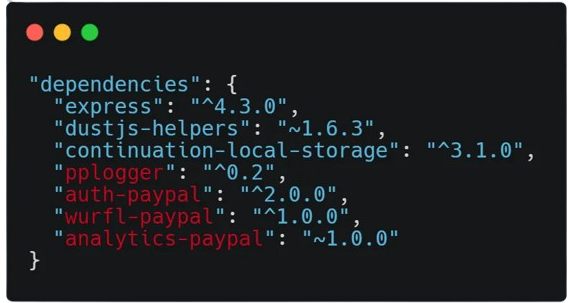
\includegraphics[width=0.5\textwidth]{imgs/image4.png}
\caption{Publicly available PayPal config file.\\
Source: Alex Birsan \cite{birsan2021dependencyconfusion}}
\label{fig:paypal-config}
\end{figure}

When a dependency manager attempts to install a package, it may encounter multiple packages sharing the same name across different repositories. Because these tools rely on predefined tie-breaking rules, such as preferring the package with the highest version number, they may unintentionally select a malicious or unintended package from a public repository rather than the legitimate internal one.

This issue becomes particularly dangerous because package names used internally are not inherently protected or reserved in public ecosystems. Even if an organization confirms that no conflicting public package exists at the time a project is created, an attacker can later publish a package with the same name to a public registry. If the attacker assigns it a higher version number or otherwise satisfies the dependency manager's resolution rules, the malicious package may be installed automatically during routine builds or updates, creating an opportunity for arbitrary code execution within the organization's environment.

The risk is further compounded by common practices such as exposing internal package names in configuration files or build artifacts, which can inadvertently reveal targets to potential attackers. We see this happening in Figure \ref{fig:paypal-config}. Similarly, abandoned or unused package names may be claimed and repurposed for malicious ends. Dependency confusion exploits these systemic weaknesses, underscoring the importance of strict namespace control, repository prioritization, and secure configuration of dependency managers to ensure that trusted internal packages are consistently preferred over unverified public sources.

\section{Why Existing Trust Models Fail}

Most ecosystems already provide standard support for identifying dependency confusion. However, these ecosystems are, in general, naive in their approach and still do leave many vulnerabilities, as evident by the exploits of Birsan. Current solutions for dependency confusion rely primarily on SBOM and configuration file analysis.

In SBOM-based analysis, a provided Software Bill of Materials is examined to extract component identifiers, such as those defined by the Common Platform Enumeration, and compare them against known databases. This process helps detect inconsistencies or unexpected components that may indicate confusion between private and public packages.

When an SBOM is not available, configuration file analysis offers a practical alternative by extracting dependency information directly from project files. Tools like Apache Maven, for instance, allow dependencies to be identified through attributes such as names and versions, which can then be used to construct a dependency tree. This tree is compared against public repositories and vulnerability databases to determine whether any dependencies could be resolved from unintended sources.

Despite their usefulness, both methods have notable limitations. SBOM analysis depends heavily on the completeness of the provided data, while configuration analysis may overlook implicit or dynamically resolved dependencies. Furthermore, both approaches rely on existing records and cannot reliably detect newly introduced malicious packages or enforce correct dependency resolution, which limits their effectiveness when used in isolation.

\section{Risk Assessment by Source Tree Matching}

To cater to the above challenges, Ding \textit{et al.} proposed source tree matching for systematic risk assessment of dependency confusion. Their method is known as ComChecker. This enables the comparison of intended components with actual resolved dependencies even in obfuscated settings \citep{ding2024dependency}. The paper focuses on Python and Java source codes, since their bytecodes can easily be decompiled.

First, by traversing the root directory, the method analyzes the specific structure of the code files and determined their types. During the resource location process, ComChecker prioritizes the use of source code for analysis if the code was provided in source code form, and otherwise does decompilation.

The source code is parsed into a structured tree representation using Python's built-in \texttt{ast} module, which allows key elements such as imports, function definitions, class definitions, and function calls to be extracted. A similar parsing process is applied to known components retrieved from public repositories such as \texttt{PyPI}, enabling the construction of comparable code structures. By analyzing and comparing these trees, it becomes possible to map source code to specific external packages and identify discrepancies or unexpected matches that may point to dependency confusion risks.

To improve efficiency, the generated AST is refined by retaining only the node types most relevant to component identification, including imports, function and class definitions, calls, and assignments, while discarding less informative nodes that contribute little to dependency analysis. This reduction lowers computational overhead and improves scalability, particularly for large projects. That said, the method is not without its limitations. It may overlook subtle behavioral differences between legitimate and malicious packages, and its effectiveness depends on how closely the structural patterns of the compared codebases align. Moreover, the optimization process, while necessary for performance, may discard contextual details that could prove relevant in more thorough security analysis.

\begin{figure}[htbp]
\centering
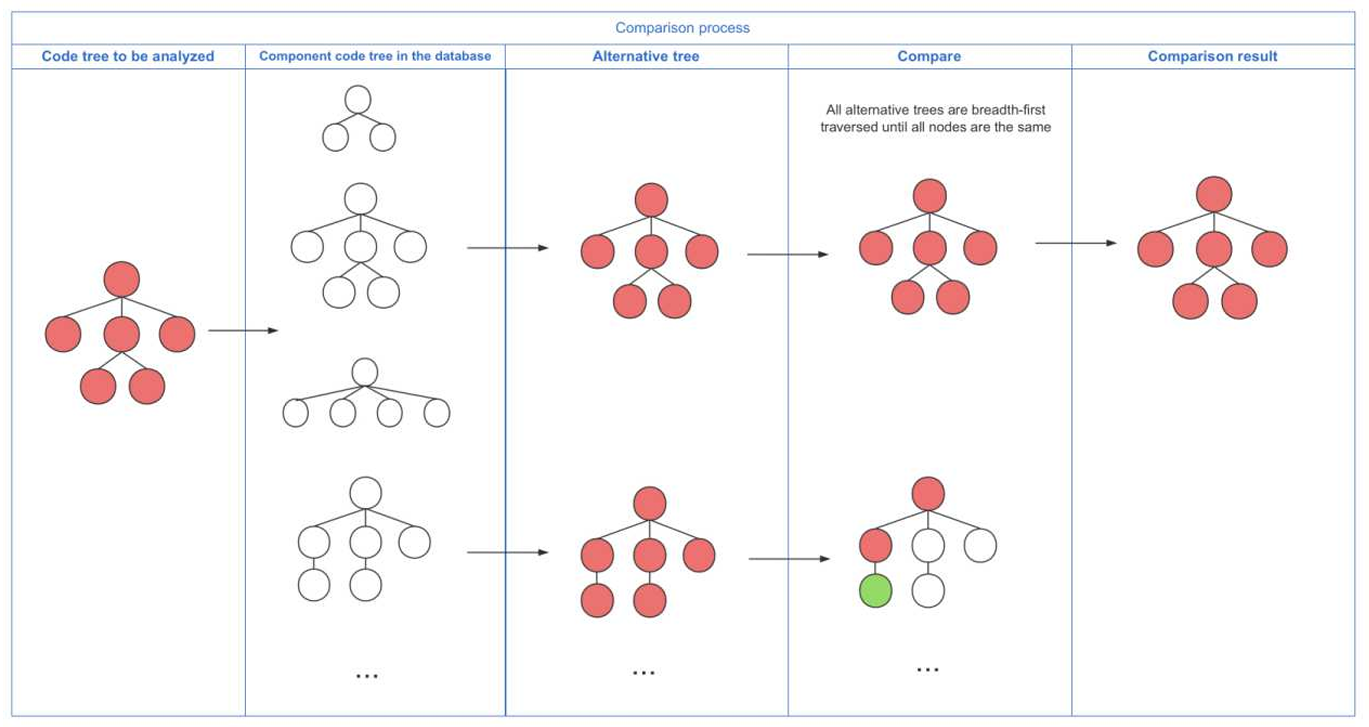
\includegraphics[width=0.96\textwidth]{imgs/image5.png}
\caption{Comparison process of code tree \\
Source: Ding \textit{et al.}, ICFTIC 2024, Fig.~4\citep{ding2024dependency}.}
\label{fig:code-tree-comparison}
\end{figure}

The final step is to actually compare, where code trees of different components in the database are compared to the code tree queried, i.e. to be analyzed. During the comparison of alternative trees, a breadth-first traversal strategy is followed. First, the node information of the first layer of child nodes is compared. If all the first level child nodes are the same, the comparison continues recursively to the next level until the end of the tree or different nodes are found. As soon as a mismatched node is found during the comparison process, we immediately stop the  comparison of the current alternative tree and start the comparison of the next alternative tree instead. This process is summarized via \ref{fig:code-tree-comparison}.

\section{Method Summary}

\begin{enumerate}
\item obtain source and component context;
\item generate abstract syntax trees;
\item optimize trees by removing low value nodes;
\item compare AST structures for accurate component mapping.
\end{enumerate}

\chapter{Existing Solution}
\label{ch:existing-solution}

\section*{Declaration of Contributions}
This chapter was prepared primarily by Parth Baranwal,
with technical inputs from the full group.

\section{Major Directions in Supply Chain Mitigation}
 
\subsection{Software Bill of Materials (SBOM) and Transparency}
 
One of the most practical first steps an organisation can take is mandating the generation and maintenance of a \textit{Software Bill of Materials} (SBOM) i.e. a structured, nested inventory of every component, library, and transitive dependency shipped within a software product. When a high severity vulnerability is publicly disclosed (such as the Log4Shell vulnerability in Log4j), teams with an accurate SBOM can immediately determine which of their services are affected and prioritise remediation accordingly, rather than conducting a time-consuming manual audit under pressure.
 
\subsection{Build Integrity and Attestation (SLSA)}
 
Even a clean codebase can be compromised if the build pipeline itself is tampered with. The \textit{Supply chain Levels for Software Artifacts} (SLSA) framework addresses this by treating the build system as a security boundary. Under SLSA, each build produces a cryptographically signed \textit{attestation} which is a verifiable record stating that a specific version of the source code was compiled in a clean, ephemeral environment and that the resulting artifact was not modified in transit before arriving in the container registry. This makes it considerably harder for an attacker to silently inject code between the repository and deployment.
 
\subsection{Zero Trust Architecture and Micro segmentation}
 
A Zero Trust approach discards the assumption that anything inside the network perimeter is inherently safe. Instead, it proceeds from the premise that the environment is already compromised, and enforces strict, identity based policy at every communication boundary. In practice, this means that even if a backdoored dependency \textit{does} execute in production, it cannot reach out to an attacker's command and control (C2) server, nor can it move laterally toward a database because it possesses neither the cryptographic identity nor the explicit policy permission required to establish those connections. Micro segmentation confines the blast radius of any individual compromise.
 
\subsection{Runtime Observability and Enforcement}
 
Many sophisticated attackers rely on what the security community calls \textit{living off the land} techniques: rather than introducing conspicuous malware, they repurpose legitimate system utilities like shell interpreters, network tools, package managers to carry out their objectives. Detecting this behaviour requires observing what software actually \textit{does} at runtime, not merely what it was expected to do. This is the domain in which eBPF technology has emerged as the pre eminent tool.
 
\section{eBPF: Architecture and Capabilities}
 
\subsection{What is eBPF?}
 
\textit{Extended Berkeley Packet Filter} (eBPF) is a kernel technology that allows purpose built, sandboxed programs to run directly inside the Linux kernel without requiring kernel source modifications or the loading of potentially unsafe kernel modules. Historically, achieving deep system observability required either slow user-space tooling or the use of kernel modules that, if defective, could destabilise the entire host. eBPF offers a third path: safe, high performance instrumentation that operates at the kernel level.
 
\subsection{Internal Architecture}

\begin{figure}[H]
    \centering
    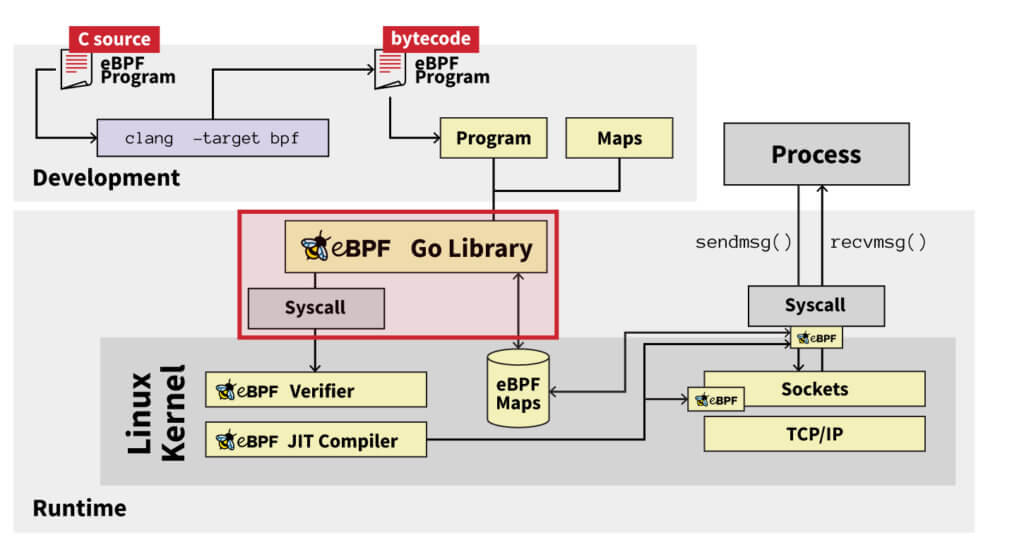
\includegraphics[width=0.85\textwidth]{imgs/image_ebpf.jpg}
    \caption{High level architecture of the eBPF subsystem in the Linux kernel.\\
Source: Red Canary \cite{redcanary2023ebpf}}
    \label{fig:ebpf_architecture}
\end{figure}
 
The eBPF subsystem consists of four principal components that work in concert:
 
\begin{itemize}[leftmargin=1.5em]
    \item \textbf{Hooks} eBPF programs are event driven. They are attached to specific points in the kernel, known as \textit{hooks} such as system call entry and exit points, network packet processing paths, and individual kernel function boundaries.
 
    \item \textbf{The Verifier} Before any eBPF program is permitted to execute, the kernel subjects it to a static analysis pass. The verifier confirms that the program cannot loop indefinitely, cannot crash the kernel, and can only access memory regions it is explicitly authorised to read or write. Programs that fail verification are rejected outright.
 
    \item \textbf{JIT Compiler} Once verified, the eBPF bytecode is translated by a \textit{Just In Time} (JIT) compiler into native machine code for the host architecture. This step ensures that the overhead imposed by an eBPF program is kept to a minimum, in many cases approaching the performance of natively compiled kernel code.
 
    \item \textbf{Maps} eBPF maps are efficient, kernel resident key value stores that serve as the primary communication channel between an eBPF program running in the kernel and the management or alerting application running in user space.
\end{itemize}
 
\section{eBPF in the Context of Supply Chain Attack Mitigation}
 
\subsection{Runtime Visibility}
 
eBPF based observability tools such as Falco and Tracee function as a kind of black box recorder for production workloads, surfacing forensic detail that conventional application logs typically cannot provide:
 
\begin{itemize}[leftmargin=1.5em]
    \item \textbf{Unexpected process execution} By attaching to the \texttt{execve} system call, an eBPF program can immediately detect anomalous behaviour, for example, a web server process spawning a shell (\texttt{/bin/sh}) or launching a cryptocurrency miner, both of which are strong indicators of active exploitation.
 
    \item \textbf{Network anomalies} eBPF can observe socket creation at the kernel level. Even when application traffic is encrypted over TLS, the act of establishing an outbound connection to an unrecognised IP address is visible and can be flagged or blocked before the handshake completes.
 
    \item \textbf{File integrity monitoring} Every \texttt{open} or \texttt{write} syscall targeting sensitive paths like \texttt{/etc/shadow}, authorised SSH key files, or critical configuration directories can be logged with full process lineage, giving security teams a precise record of which process attempted which access and when.
\end{itemize}
 
\subsection{Runtime Enforcement}
 
More recent tooling, notably Tetragon, extends eBPF's role from passive observation to active enforcement. Because eBPF logic executes synchronously within the kernel call path, it can intervene before a potentially harmful action is completed:
 
\begin{itemize}[leftmargin=1.5em]
    \item \textbf{Synchronous system call blocking} An eBPF enforcement program can intercept a disallowed syscall and return an error to the calling process, preventing the action from taking effect entirely without any additional userspace round trip.
 
    \item \textbf{Process termination} Should a backdoored dependency attempt to escalate its privileges, an eBPF program can immediately deliver a \texttt{SIGKILL} to that specific process, containing the threat without disrupting co-located workloads or requiring a full node reboot.
 
    \item \textbf{Dynamic network policy injection} If a container begins exhibiting lateral movement behaviour; for example, scanning internal subnets for open ports; its network traffic can be dropped at the kernel level in real time, effectively quarantining the workload without manual intervention.
\end{itemize}
 
\section{Why eBPF is Particularly Suited to Supply Chain Threats}
 
A critical advantage of eBPF based security is its positional authority. Because the enforcement logic runs inside the kernel, it occupies a layer below every application, library, and runtime that an attacker might seek to subvert. Any instruction that a malicious payload issues no matter however it was introduced, and however it is obfuscated must eventually pass through the kernel to interact with the system. This structural property makes eBPF based controls exceptionally difficult to evade, and distinguishes them from conventional security agents that operate in user space alongside the very processes they are trying to monitor.


\chapter{Proposed Solution}
\label{ch:proposed-solution}

\section*{Declaration of Contributions}
This chapter was jointly prepared by Parth Baranwal and Utkarsh Kumar, with review support from Tanay Kapadia.

\section{Background: Symbolic Execution}
 
Before describing the full validation pipeline, it is worth grounding the reader in what symbolic execution actually is, since the rest of the proposal builds directly on it.
 
\subsection{What Is Symbolic Execution?}

 
In ordinary program testing, you run a piece of code with specific, concrete inputs for example, the string \texttt{"User123"} or the integer \texttt{42} and observe what happens. This is fast and intuitive, but it is fundamentally limited: you can only observe the paths that your chosen inputs happen to trigger. Hidden backdoors, logic bombs, or time gated conditions that require a very specific input may never be exercised by any reasonable test suite.
 
Symbolic execution takes a different approach. Instead of supplying a concrete value, the engine replaces each input with a \textit{symbolic variable} i.e. a mathematical placeholder, say $\alpha$ or $\beta$ and then propagates that symbol through the computation. As the engine steps through the code, it maintains a \textbf{path condition}: a logical formula that accumulates the constraints that must be true for the execution to have followed that particular sequence of branches.

\hyperref[fig:symex]{Figure 8.1} shows how we work around conditional jumps when performing symbolic execution.

\begin{figure}[H]
    \centering
      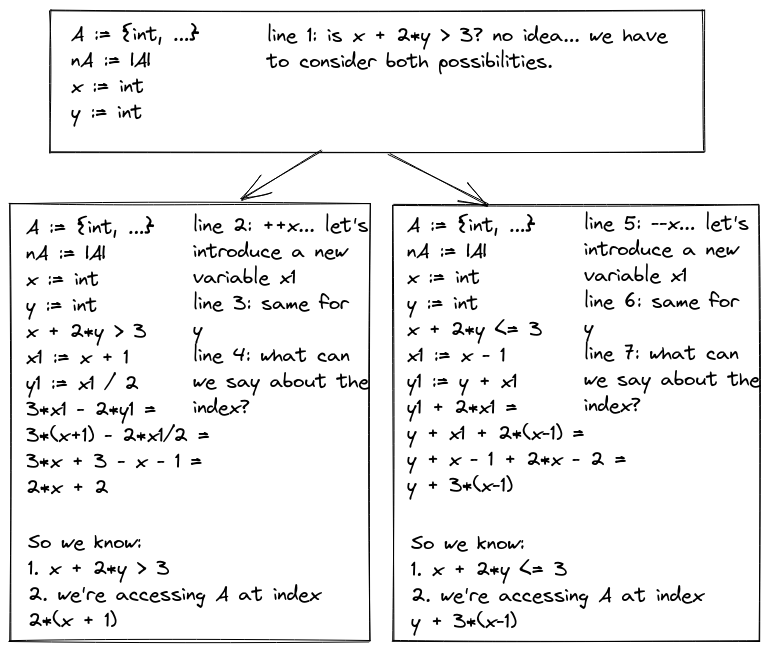
\includegraphics[width=0.85\textwidth]{imgs/symex.png}

    
    \caption{Path constraint propagation over conditional jumps.\\
Source: Michael McTernan \cite{mcternan_symex}}
    \label{fig:symex}
\end{figure}
\subsection{A Concrete Illustration}
 
Consider the following minimal Python fragment:
 
\begin{lstlisting}[caption={A simple function with a hidden condition}]
def process(user, secret_key):
    if user == "admin_backup":
        if secret_key == 0xDEADBEEF:
            exfiltrate_credentials()   # malicious branch
    normal_operation()
\end{lstlisting}
 
A conventional test suite calling \texttt{process("alice", 123)} would never reach \texttt{exfiltrate\_credentials()}. A symbolic execution engine, however, introduces $\alpha$ for \texttt{user} and $\beta$ for \texttt{secret\_key} and explores \textit{all} branches simultaneously. It discovers the path:
 
\[
    \pi_{\text{malicious}} : \quad \alpha = \texttt{"admin\_backup"} \;\wedge\; \beta = \texttt{0xDEADBEEF} \;\Rightarrow\; \texttt{exfiltrate\_credentials()}
\]
 
This path condition is then handed to an SMT solver, which checks whether there \textit{exist} concrete values for $\alpha$ and $\beta$ that satisfy it. In this case, the answer is obviously yes---and the engine has found the hidden branch without ever having to guess the magic inputs in advance.
 
\subsection{SMT Solvers and Their Role}
 
An SMT solver is a tool that decides, given a logical formula over variables drawn from various mathematical theories (integers, bit vectors, arrays, strings, and so on), whether the formula is \textit{satisfiable} i.e., whether there is any assignment of values to the variables that makes it true. Well known solvers include Microsoft's \textbf{Z3} and Stanford's \textbf{CVC5}.
 
In the context of supply chain security, the SMT solver serves two roles:
 
\begin{enumerate}
    \item \textbf{Feasibility checking:} Pruning paths whose constraints are mathematically impossible (e.g., $\alpha > 5 \;\wedge\; \alpha < 3$), so the engine does not waste time exploring dead branches.
    \item \textbf{Semantic matching:} Determining whether a path condition derived from an unknown binary is \textit{logically equivalent} to, or a \textit{generalisation of}, a known malicious behaviour.
\end{enumerate}
 
 
% ============================================================
\section{Proposed Solution: Semantic Supply Chain Validation}
 
The core idea is to treat a software component not as a flat sequence of instructions, but as a \textit{collection of mathematical paths}. By converting those paths into SMT formulae, we can prove whether a component contains behaviours that matches known malicious patterns, regardless of how the code has been obfuscated or repackaged.
 
\subsection{Technical Workflow}
 
The pipeline consists of four sequential stages:
 
\begin{enumerate}
 
    \item \textbf{Path Exploration} A symbolic execution engine ingests the compiled binary. It replaces all external inputs (command line arguments, environment variables, network data) with symbolic variables $\alpha, \beta, \gamma, \ldots$ and systematically traverses the control flow graph, forking at every conditional branch.
 
    \item \textbf{Equation Generation} At every exit point, whether a return statement, a system call, or an abnormal termination, the engine serialises the current path condition as an SMT formula. This formula encodes both the \textit{conditions} required to reach that exit and the \textit{system state} (register values, memory contents, file handles) at the moment of arrival.
 
    \item \textbf{Corpus Matching} The generated formulae are queried against a curated database of \textbf{Malicious Semantic Signatures}: mathematical representations of behaviours such as ``unauthorised credential exfiltration,'' or ``covert network backdoor.'' Matching is performed via structural hashing and logical subsumption rather than byte level comparison.
 
    \item \textbf{Reporting} Any path whose formula is found to subsume a malicious signature is escalated as a critical finding, with a full backtrace indicating the sequence of branches that leads to the offending behaviour.
 
\end{enumerate}
 
\subsection{Pseudocode: Semantic Matcher}
 
\hyperref[lst:matcher]{Listing B.1} presents the core matching logic with added annotations to explain the purpose of each major block.
 
 
\section{Advantages of the Symbolic Approach}
 
\subsection{Exhaustive Path Coverage}
Dynamic testing can only observe code paths that are actually exercised by the chosen test inputs. Symbolic execution, by contrast, explores \textit{all feasible} paths simultaneously. A backdoor that activates only when the current date is 2026-01-01, or only when a particular administrator credential is present, will be discovered and its path condition will be generated even though no test suite would ever hit it deliberately.
 
\subsection{Resilience to Code Obfuscation}
Attackers routinely rename variables, insert dead code, or apply packing and encryption to defeat signature scanners. Because SMT matching operates on the \textit{logical meaning} of a path, for example, ``if condition $A$ and $B$ hold, send file $C$ to address $D$'' the mathematical signature is invariant to superficial code transformations. Renaming a variable from \texttt{x} to \texttt{tmp\_74f3} does not change the resulting formula.
 
\subsection{Detection of Logic Bombs}
Logic bombs are a particularly insidious form of malicious code because they lie entirely dormant until a specific precondition is met. Symbolic execution is ideally suited to finding them: the engine will systematically explore the branch guarded by \texttt{if system\_user == "admin\_backup"}, generate an SMT formula for it, and flag the match if the formula corresponds to a known malicious pattern. Standard runtime monitoring would never see this branch execute in a normal deployment.
 
\subsection{Proactive ``Shift Left'' Security}
The entire analysis runs on the binary artifact before it is ever deployed. This means the validation can be integrated directly into a CI/CD pipeline, vetting every third-party library update at the point of ingestion rather than waiting for anomalous behaviour to surface in production.
 
\section{Addressing the Limitations}
 
The primary practical challenge is \textbf{path explosion}: as the number of conditional branches grows, the number of distinct paths grows exponentially. Combined with the inherent computational cost of SMT solving, this makes exhaustive analysis of large binaries prohibitive.
 
We propose a \textbf{Triage Model} to manage this cost pragmatically:
 
\begin{table}[H]
\centering
\renewcommand{\arraystretch}{1.4}
\begin{tabular}{@{}lll@{}}
\toprule
\textbf{Mechanism} & \textbf{Scope} & \textbf{Trigger Condition} \\
\midrule
eBPF Runtime Monitoring & All dependencies & Always on; low overhead \\
Symbolic SMT Analysis & Core / high risk dependencies & On ingestion or version bump \\
\bottomrule
\end{tabular}
\caption{Proposed triage model: lightweight runtime observability for broad coverage; deep symbolic analysis reserved for critical components.}
\label{tab:triage}
\end{table}
 
Under this model, eBPF probes provide continuous, low overhead behavioural monitoring across the full dependency graph. Deep symbolic analysis is reserved for components that are either (a) direct dependencies of security critical subsystems, or (b) flagged by the eBPF layer as exhibiting anomalous behaviour. This keeps the computational budget tractable while maintaining strong assurances where they matter most.
 
Additional mitigations for path explosion include: loop bounding (limiting the number of times any loop is unrolled symbolically), lazy initialisation of memory regions, and compositional analysis (analysing library functions once and caching their summaries for reuse).

\chapter{Conclusion}
\label{ch:conclusion}

\section*{Declaration of Contributions}
This chapter was jointly prepared by Parth Baranwal and Adesh Palkar,
with final review by all Group 4 members.

This report examined modern cyber threats and focused on software supply chain attacks
as a high impact, trust centric threat model. Through the XZ Utils case study and related
research synthesis, we observed that a single compromised upstream dependency can propagate
risk to many downstream systems.

The central conclusion is that dependency trust must be continuously verified, not implicitly
assumed. Existing controls improve visibility and reduce risk, but robust defense requires
layered safeguards across package publication, dependency resolution, CI/CD pipelines,
and runtime monitoring.

\section{Future Work}

The following directions are recommended for improving practical defenses:

\begin{enumerate}
\item standardized provenance and signed artifact verification across package ecosystems;
\item stronger CI/CD policy gates for dependency updates and transitive risk checks;
\item scalable hybrid analysis (static + dynamic + symbolic) with low false positive rates;
\item faster ecosystem wide notification and coordinated mitigation for exposed dependents;
\item broader adoption of security by default package publishing and maintainer hardening.
\end{enumerate}

